% !TEX TS-program = xelatex
% !TEX encoding = UTF-8 Unicode
\documentclass[10pt,aspectratio=1610]{beamer}
%\documentclass[10pt]{beamer}

\usetheme[progressbar=frametitle]{metropolis}
\usepackage{appendixnumberbeamer}


\usepackage{booktabs}
\usepackage[scale=2]{ccicons}

\usepackage{pgfplots}
\usepgfplotslibrary{dateplot}

\usepackage{xspace}

\usepackage{bm}

% Color definitions 
%\usepackage[dvipsnames]{xcolor}

% Remove "Figure #" from figures
\setbeamertemplate{caption}{\raggedright\insertcaption\par}

% Custom commands
% Metropolis theme name 
\newcommand{\themename}{\textbf{\textsc{metropolis}}\xspace}

% Derivatives
\newcommand{\pfrac}[3][]{\frac{\partial^{#1} #2}{\partial #3^{#1}}}
\newcommand{\dd}[3][]{\frac{\mathrm{d}^{#1} #2}{\mathrm{d} #3^{#1}}}
\newcommand{\pp}[2][]{\partial^{#1}_{#2}}


\newcounter{example}
\stepcounter{example}
\newcounter{exercise}
\stepcounter{exercise}

\renewcommand{\vec}{\mathbf}
\newcommand{\varone}{\vec{x}}
\newcommand{\argone}{(t,\varone)}
\newcommand{\R}{\mathbb{R}}
\newcommand{\CC}{\mathbb{C}}
\newcommand{\Q}{\mathbb{Q}}
\newcommand{\Z}{\mathbb{Z}}
\newcommand{\N}{\mathbb{N}}
\newcommand{\norm}[1]{\left\lVert#1\right\rVert}
\newcommand{\fone}{\vec{f}}
\newcommand{\ftwo}{\vec{g}}
\newcommand{\fthr}{\vec{h}}
\newcommand{\ffor}{\bm{\phi}}
\newcommand{\opone}{\mathcal{L}}
\newcommand{\optwo}{\mathcal{G}}
\renewcommand{\Re}{\operatorname{Re}}
\newcommand{\iprod}[2]{\langle #1,#2 \rangle}
\newcommand{\diff}{\mathrm{d}}
\newcommand{\fouriert}{\mathcal{F}}

\title{On stability of numerical schemes}
\subtitle{How to discretize time for some problems}
\date{16/2/2021}
\date{}
%\author{18.303 Linear Partial Differential Equations: Analysis and Numerics}
\institute{18.303 Linear Partial Differential Equations: Analysis and Numerics}
\titlegraphic{\hfill
\includegraphics[height=2em]{../MIT-logo.pdf}}

\begin{document}
	
	\maketitle
	
%	\begin{frame}{Table of contents}
%		\setbeamertemplate{section in toc}[sections numbered]
%		\tableofcontents%[hideallsubsections]
%	\end{frame}

\begin{frame}{Behavior of time-dependent problems}
	Let us consider the differential equation
	\[  
	\alpha \pfrac[2]{u\argone}{t} + \mu \pfrac{u\argone}{t} = \opone u\argone
	\]
	with some boundary conditions that we will not specify at this point. Here we assume $ \alpha, \mu \geq 0 $.
	
	\pause
	We assume that $ \opone $ has a complete eigenbasis $ \{ \eigtwo \} $ with
	\[  
	\opone \eigtwo (\vec{x}) = \eigvone \eigtwo (\vec{x})
	\] 
	and
	\[  
	u\argone = \sum_{\vec{n}} \coefone(t) \eigtwo(\vec{x}).
	\]
\end{frame}

\begin{frame}
	Plugging the expansion of $ u $ in the differential equation and using the \emph{linear independence} of $ \eigtwo $ gives 
	\[  
	\alpha \pfrac[2]{\coefone(t)}{t} + \mu \pfrac{\coefone(t)}{t} = \eigvone \coefone(t).
	\]
	This equation is solved by an exponential ansatz 
	\[ \coefone = \exp(a_\vec{n} t). \]
	
	\pause
	Plugging this in gives the characteristic equation
	\[ \left( \alpha a_\vec{n}^2 + \mu a_\vec{n} - \eigvone \right) \exp(a_\vec{n} t)  = 0, \]
	which can be solved giving
	\[ a_\vec{n} = \frac{-\mu \pm \sqrt{\mu^2 + 4 \alpha \eigvone}}{2\alpha} \]
	if $ \alpha \neq 0 $
	and 
	\[ a_\vec{n} = \frac{\eigvone}{\mu} \]
	otherwise. 
\end{frame}

\begin{frame}{Case i: $ \alpha = 0 $}
	This describes first order dynamic. The solution of the $ \vec{n}th $ coefficient is proportional to
	\[ \exp\left( \frac{\eigvone}{\mu} t \right). \]
	
	\pause
	Depending on the sign of $ \eigvone $ this solution is either growing or decreasing exponentially. 
	
	\pause
	Note: remember that the eigenvalues of the Laplacian are negative (semi)definite. The modes with the zero eigenvalue are constant in time and the rest of them decrease. This is the case for the heat equation. See how important it is that the eigenvalues are negative?
\end{frame}

\begin{frame}{Case ii: $ \mu = 0 $}
	This gives a kind of wave equation. Now the solution is 
	\[ \exp\left(\pm \sqrt{\frac{\eigvone}{\alpha}} t \right). \]
	
	Again, if \emph{all} the eigenvalues are negative, the solution will be oscillating. Otherwise there will be a solution (for each $ \vec{n} $) that is decaying and a solution that grows exponentially. We also have the special case $ \eigvone = 0 $ for modes that do not change in time. 
\end{frame}

\begin{frame}{General case}
	\[  
	\coefone(t) \propto \exp \left(
	\frac{-\mu \pm \sqrt{\mu^2 + 4 \alpha \eigvone}}{2\alpha} t
	\right)
	\]
	
	\pause
	If we assume that $ \alpha \neq 0 $ we can write this as 
	\[  
	\coefone(t) \propto \exp \left(
	\frac{-\mu \pm \sqrt{\mu^2 + 4 \eigvone}}{2} t
	\right) =  \exp \left(
	\frac{-\mu t}{2} \right) \exp \left( \pm \frac{\sqrt{\mu^2 + 4 \eigvone}}{2} t
	\right)
	\]
	with the rescaling $ \mu \to \mu/\alpha $ and $ \eigvone \to \eigvone/\alpha $ (if we were careful here, we would use different symbols for these new coefficients but let's allow us to be a bit lazy).
\end{frame}

\begin{frame}
	\[  
	\coefone(t) \propto  \exp \left(
	\frac{-\mu t}{2} \right) \exp \left( \pm \frac{\sqrt{\mu^2 + 4 \eigvone}}{2} t
	\right)
	\]
	\begin{figure}
		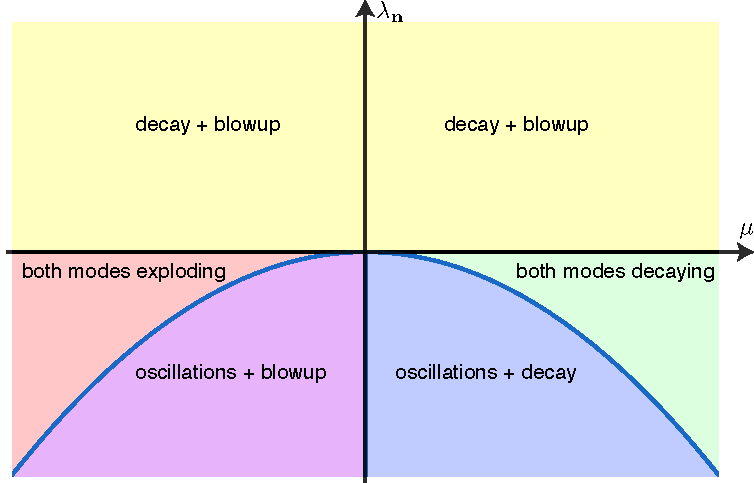
\includegraphics[width=0.7\textwidth]{phase_diagram}
		\caption{Diagram of different behavior}
	\end{figure}
\end{frame}

\begin{frame}{Stability}
	\begin{itemize}[<+->]
		\item Stability of time-dependent numerical solutions can mean many things
		\item Something that is \emph{always} required is that the solutions do not blow up unphysically (e.g. the solution to the heat equation doesn't blow up)
		\item Many times we use scalar quantities like the energy to see if the numerical solution agrees with known behavior of the equation
		\item For example:
		\begin{itemize}
			\item Wave equations are \emph{energy conserving} 
			\item For heat equations energies are non-increasing
		\end{itemize}
		\item We will get back to energies later; for now we'll concentrate on stability in the sense that the solutions don't blow up
	\end{itemize}
\end{frame}

\begin{frame}
	Let us look at a heat equation with 
	\[ \pfrac{u\argone}{t} = \opone u\argone \]
	with some sufficient boundary conditions.
	
	\pause
	Assume that we discretize the function in time (but not in space, for now). We introduce a time step $ s $ and function values \[ \ftime{k} (\vec{x}) = u(ks,\vec{x}). \] 
	
	\pause
	Forward difference will give
	\[ \frac{\ftime{k+1}-\ftime{k}}{s} = \opone \ftime{k}. \]
	
\end{frame}

\begin{frame}
	We write this in the eigenbasis of $ \opone $ as 
	\[ \frac{\eigtime{k+1}-\eigtime{k}}{s} = -\eigvone \eigtime{k}. \]
	
	\pause
	Solving for $ \eigtime{k+1} $ gives
	\[ \eigtime{k+1} = (1 - s \eigvone) \eigtime{k}. \]
	
	\pause
	This recursion relation is easy to solve giving
	\[ \eigtime{k} = (1 - s \eigvone)^{k} \eigtime{0}. \]
	
	\pause
	We can easily see that this is bounded if $ |1 - s \eigvone| < 1 $. 
	
	\pause
	For physical systems, the eigenvalues are negative ($ \eigvone > 0 $) and we only have to worry about the most negative eigenvalue in the system. 
	
	\pause
	Assume we have some \emph{truncated} basis with $ N $ eigenvectors. We assume $ \lambda_N $ to be the largest eigenvalue (by absolute value). Now we get the condition
	\[ 1 - s \lambda_N > -1  \Leftrightarrow s < 2/\lambda_N. \]
\end{frame}

\begin{frame}{What if we also have spatial discretization?}
	\pause
	We will just have a matrix substitution $ \opone \to L $ with some matrix $ L $. It will have its own eigenbasis and associated eigenvalues.
	
	\pause
	\textbf{Exercise:} Assume $ \opone = \Delta $ (the Laplacian). Assume we have Dirichlet boundaries for the heat equation. Now 
	
	\[  
	A = \frac{1}{\Delta x^2} \begin{pmatrix}
		 -2 & 1  &   &  &  \\
		1 & -2 & 1  &   &    \\
		&  \ddots & \ddots & \ddots  &  \\
		& & 1 & -2 & 1 \\
		& & & 1 & -2 
	\end{pmatrix}.
	\]
	
	What is the stability condition for the time step?
\end{frame}

\begin{frame}
	The eigenvectors of $ A $ are $ \phi_n(k) = \sin(n k \pi/(N+1)) $ and the associated eigenvalues are 
	$$ -2\cdot\frac{1-\cos(n\pi/(N+1))}{\Delta x^2}. $$
	
	\pause
	The largest eigenvalue comes with $ n = N $, which, for large $ N $, we can approximate as
	$$ -2(1-\cos(N\pi/(N+1))) \approx -2(1 - \cos(\pi)) = -4. $$
	
	\pause
	This gives $ \lambda_N \approx 4/\Delta x^2. $ Now the condition becomes 
	\[  
	s < 2/\lambda_N = \Delta x^2/2.
	\]
	
	\pause
	This is called the Courant–Friedrichs–Lewy (CFL) condition. For those of you who did Pset 1, you probably noticed that the time step had to be very small. This explains why.
\end{frame}

\begin{frame}
	Let's try something else. Let's discretize the time as 
	\[ \frac{\ftime{k+1} - \ftime{k}}{s} = \frac{\opone \ftime{k} +  \opone \ftime{k+1}}{2}. \]
	
	\pause
	This is called the Crank-Nicolson method. It's equivalent to using central difference for time at time $ k+1/2 $. For the coefficients we get 
		\[ \frac{\eigtime{k+1} - \eigtime{k}}{s} = -\lambda_n \frac{ \eigtime{k} +  \eigtime{k+1}}{2}. \]
	
	\pause
	Solving for $ \eigtime{k+1} $ gives 
	\[ \eigtime{k+1} = \left(
	\frac{1 - \lambda_n s/2 }{1 + \lambda_n s/ 2}
	\right) \eigtime{k} \]
	
\end{frame}

\begin{frame}
	Assume $ \lambda_N > 0 $ (negative definite operator). 
	
	\pause
	Solving for the condition gives
	\[ \left|
	\frac{1 - \lambda_n s/2 }{1 + \lambda_n s/2}
	\right| < 1, \]
	which we can write as 
	\[ -1 < \frac{1 - \lambda_n s/2 }{1 + \lambda_n s/2} < 1. \]
	
	\pause
	The lower bound gives $ -1 < 1 $ while the upper bound gives $ -\lambda_n < \lambda_n $, which is always true if $ \lambda_n > 0 $. 
	
	\pause
	We see that this method is \alert{unconditionally stable} i.e. the stability doesn't depend on $ s $ if we would do the spatial discretization.
	
	\pause
	\alert{Word of warning:} stability just means here that the discretized system doesn't blow up. We should still make $ s $ sufficiently small if we want to approximate the time evolution well. 
	
\end{frame}

\end{document}
